\documentclass[preprint,12pt,authoryear]{elsarticle}
% Draft of the main article (see esboco_artigo.md for the outline and the list of calculations).
% Compile: pdflatex artigo && pdflatex artigo. Figures: figuras/ (scripts/figuras_artigo.py of Projects/SlopeRainfall).
\usepackage[T1]{fontenc}
\usepackage[utf8]{inputenc}
\usepackage{lmodern}
\usepackage{amsmath,amssymb,bm}
\usepackage{booktabs,multirow}
\usepackage{graphicx}
\usepackage[hidelinks]{hyperref}
\usepackage{lineno}
\usepackage{xcolor}
\usepackage[margin=2.5cm]{geometry}
\graphicspath{{figuras/}}
\newcommand{\Ic}{I_c}
\newcommand{\kpa}{\,\mathrm{kPa}}
\newcommand{\mmh}{\,\mathrm{mm/h}}
\newcommand{\pend}[1]{\textcolor{red}{#1}}
\linenumbers

\journal{Engineering Geology}

\begin{document}
\begin{frontmatter}

\title{Critical rainfall intensity of unsaturated slopes: how much do uncoupled, passive-air analyses overestimate
it?}

\author[ufpr]{Diogo Lira Cecilio\corref{cor}}
\ead{cecilio.diogo@gmail.com}
\cortext[cor]{Corresponding author}
\affiliation[ufpr]{organization={[affiliation]}, country={Brazil}}

\begin{abstract}
Physically based rainfall thresholds for unsaturated slopes usually come from uncoupled seepage analyses with
atmospheric pore air followed by stability analyses at successive instants. We quantify how these hypotheses bias the
rainfall that triggers failure. A coupled formulation with displacement, pore-water and pore-air pressures (Bishop's
effective stress, Mohr--Coulomb plasticity) is implemented in the open-source library NeoPZ and validated against the
Liakopoulos drainage test; the factor of safety (FS) is obtained by strength reduction with frozen pressures. Since
values below one are not physical states, models are compared by the critical intensity $I_c$ of a 24-h rainfall,
the smallest that brings the FS to one, and by the time to failure. For the slope of Rahardjo et al.\ (2007) with
$k_s=36$~mm/h, the uncoupled, passive-air model gives $I_c=48$~mm/h ($1.3k_s$); the coupled model with active air
gives 31~mm/h ($0.9k_s$) with an associated flow rule and 26~mm/h ($0.7k_s$) without dilatancy. The usual hypotheses
thus overestimate the failure-triggering rainfall by 54--86\% and delay failure by up to 10~h. Their effects are
opposite: trapped air halves $I_c$, coupling raises it by 4--63\%, and the air dominates. Once the surface ponds, the
air below the wetting front is compressed to 36--38~kPa; less water infiltrates and the matric suction increases, but
the pore-water pressure follows the air pressure and the effective stress drops, so that a low-permeability slope
deemed safe under short rainfalls reaches limit equilibrium. Dilatancy shifts $I_c$ by about 20\% and decides whether
the transient collapses. The bias persists with $\chi=S_e$ and mesh refinement and vanishes when $I_c$ is well below
$k_s$.

\end{abstract}

\begin{keyword}
unsaturated slope \sep rainfall infiltration \sep pore-air pressure \sep hydro-mechanical coupling \sep dilatancy
\sep critical rainfall intensity \sep strength reduction method
\end{keyword}
\end{frontmatter}

%======================================================================
\section{Introduction}
%======================================================================

Rainfall-induced landslides in residual and colluvial soils are usually triggered by the loss of matric suction and
the rise of pore-water pressure in a shallow unsaturated zone. Warning systems rely on rainfall thresholds, empirical
\citep{caine1980,guzzetti2008} or physically based, the latter obtained by transient seepage analyses followed by
a stability analysis at successive instants. In engineering practice this chain is a seepage code solving Richards'
equation on a rigid skeleton with the pore air at atmospheric pressure (SEEP/W, HYDRUS, the hydraulic module of
PLAXIS), followed by limit equilibrium (SLOPE/W) or by strength reduction with the pore pressures of each instant
\citep{ng1998,rahardjo2007,tang2018,pradhan2022}.

The parametric study of \citet{rahardjo2007} is a reference of this approach. For a homogeneous slope they
concluded that the saturated permeability $k_s$ controls the response: there is a limiting intensity above which the
minimum factor of safety (FS) no longer decreases, a lower FS plateau of about 0.81--0.82, slopes with
$k_s\le10^{-6}$~m/s do not fail in rainfalls of up to 24~h, and the slope angle, height and initial water table are
secondary. Three hypotheses of that chain are rarely questioned together.
\begin{enumerate}
\item \emph{Atmospheric pore air.} When the ground surface ponds, the air between the wetting front and the water
table can only leave through the surface and is compressed by the infiltrating water. Laboratory columns
\citep{toumavauclin1986} and two-phase flow analyses of slopes \citep{cho2016} show that the air delays the wetting
front and that its pressure lowers the FS; these slope analyses, however, typically solve the flow on a rigid
skeleton and evaluate the stability by limit equilibrium.
\item \emph{Uncoupled seepage.} The volumetric strain of the skeleton changes the pore pressures. Coupled analyses
can give smaller FS than uncoupled ones \citep{qi2015} and have been used to back-analyse failures
\citep{yang2017}, but the comparisons are made with the minimum FS, not with the rainfall that triggers the failure.
\item \emph{Flow rule.} The coupled models that predict failure use non-dilatant soils
\citep{wang2018mpm,liu2021}, while the strength reduction method is usually applied with an associated flow rule.
Dilatancy generates suction during plastic shearing and can arrest a coupled failure; none of the studies we
reviewed varies it.
\end{enumerate}

This paper quantifies how these three hypotheses bias the critical rainfall intensity of an unsaturated slope, that
is, the smallest intensity of a rainfall of given duration that brings the slope to failure. A three-field
formulation (displacement, pore-water and pore-air pressures) is implemented in the open-source finite element library
NeoPZ \citep{devloo1997} and validated against the drainage test of \citet{liakopoulos1965}. Since a factor of
safety below one is not a physical state, the models are compared by the critical intensity $\Ic$ and the time to
failure, not by the minimum FS. The slope of \citet{rahardjo2007} is the reference case: the four combinations of
coupling and air model isolate the contribution of each hypothesis, and the effect of dilatancy, of the soil
permeability, of the Bishop parameter, of the confinement of the air and of the mesh is then assessed.

%======================================================================
\section{Formulation and implementation}\label{sec:form}
%======================================================================

\subsection{Governing equations}

The soil is a deformable porous medium with two immiscible fluids, water and air, under isothermal conditions;
grains and water are nearly incompressible and the air is an ideal gas; dissolved air and vapour are neglected.
Small strains and quasi-static equilibrium are assumed. With tension positive and pore pressures positive in
compression, the total stress is
\begin{equation}
\bm\sigma=\bm\sigma'-p_B\,\mathbf I,\qquad p_B=\chi\,p_w+(1-\chi)\,p_a, \label{eq:bishop}
\end{equation}
where $\bm\sigma'$ is Bishop's effective stress \citep{bishop1959} and $\chi$ the Bishop parameter. The unknowns are the
displacement $\mathbf u$ and the gauge pressures $p_w$ and $p_a$; the capillary pressure is $p_c=p_a-p_w$. The
balance equations of momentum, water mass and air mass are
\begin{gather}
\nabla\cdot\bm\sigma-\gamma\,\mathbf e_y=\mathbf 0,\\
\frac{nS_w}{K_w}\,\dot p_w+n\,\dot S_w+S_w\,\dot\varepsilon_v+\nabla\cdot\mathbf q_w=0,\qquad
\frac{nS_a}{p_a+p_{atm}}\,\dot p_a-n\,\dot S_w+S_a\,\dot\varepsilon_v+\nabla\cdot\mathbf q_a=0,
\label{eq:massa}
\end{gather}
with $S_a=1-S_w$, $S_w=S_w(p_c)$, $\varepsilon_v$ the volumetric strain (positive in expansion), $\gamma$ the total
unit weight, $\mathbf e_y$ the upward unit vector, a unit Biot coefficient and Darcy's law
\begin{equation}
\mathbf q_w=-\frac{k_{rw}}{\gamma_w}\,\mathbf K\left(\nabla p_w+\gamma_w\mathbf e_y\right),\qquad
\mathbf q_a=-\frac{k_{ra}}{\gamma_w}\frac{\mu_w}{\mu_a}\,\mathbf K\left(\nabla p_a+\gamma_a\mathbf e_y\right),
\end{equation}
where $\mathbf K$ is the saturated conductivity tensor, $k_{rw}$ and $k_{ra}$ the relative permeabilities and
$\mu_w/\mu_a=55.6$. The retention curve is that of \citet{fredlund1994} with the correction factor $C(\psi)=1$,
$S_w=[\ln(e+(p_c/a)^n)]^{-m}$, the water permeability is $k_{rw}=S_w^{\,4}$ \citep{leong1997} and the air
permeability follows Brooks and Corey with $\lambda=3$, $k_{ra}=(1-S_w)^2(1-S_w^{5/3})\ge k_{ra}^{\min}=10^{-4}$.

The effective stress follows the Mohr--Coulomb criterion with elastic moduli $E$, $\nu$. With an associated flow rule
($\psi=\phi'$) the return mapping is analytical, with the consistent tangent; with $\psi<\phi'$ an iterative
non-associated return mapping is used. The strength envelope of \citet{fredlund1978} with $\phi^b$ corresponds to
$\chi=\tan\phi^b/\tan\phi'$ on the suction; \citet{rahardjo2007} use $\phi^b=\phi'$, i.e.\ $\chi=1$, which is the
default here; $\chi=S_e$ is the alternative examined in Section~\ref{sec:gen}.

Four models are compared (Table~\ref{tab:modelos}). In the uncoupled models the terms $S_w\dot\varepsilon_v$ and
$S_a\dot\varepsilon_v$ are removed from Eq.~\eqref{eq:massa}, i.e.\ the flow is solved on a rigid skeleton, as in a seepage code; the
equilibrium still uses the pressures. In the passive-air models $p_a=0$ in the whole domain and the air mass balance
is not solved. Model (iii) gathers the hypotheses of \citet{rahardjo2007} and of most of the literature.

\begin{table}[htbp]
\centering\small
\caption{Models compared.}\label{tab:modelos}
\begin{tabular}{lll}
\toprule
model & coupling & air\\
\midrule
(i) complete & coupled & active ($p_a=0$ only on the ground surface)\\
(ii) & coupled & passive ($p_a=0$)\\
(iii) the usual one & uncoupled & passive\\
(iv) & uncoupled & active (two-phase flow on a rigid skeleton)\\
\bottomrule
\end{tabular}
\end{table}

\subsection{Boundary conditions}

The rainfall is a flux on the horizontal projection of the ground surface with the unilateral condition $p_w\le0$,
inflow $\le I_r$ and complementarity, solved as an active set of ponded vertices; without rainfall the same condition
is a seepage face. The pore air is atmospheric on the ground surface and the base and lateral boundaries are closed
to the air (the effect of opening them is examined in Section~\ref{sec:confinamento}). The water pressure is hydrostatic
on the lateral boundaries below the water table and the boundaries are impervious above it. The base is fixed and the
lateral boundaries are on rollers.

\subsection{Discretization and solution}

Displacements are interpolated by quadratic and pressures by linear triangles (Taylor--Hood), in plane strain. The
storage terms in $\dot S_w$ and $\dot p_a$ are lumped at the vertices in the mass-conservative secant form
$n(S^{n+1}-S^n)$ \citep{celia1990}. The equations are integrated by the implicit Euler method and solved by Newton's
method with the complete consistent Jacobian, including the derivatives of the permeabilities, of the saturation and
of $\chi$; Dirichlet conditions are eliminated and the linear systems are solved with Pardiso. A time step that does
not converge is restarted from its initial state with up to five levels of bisection. The time step is 15~min during
the rainfall, 1~h in the following 24~h and 4~h afterwards.

\subsection{Factor of safety}\label{sec:fs}

At selected instants an independent stability analysis is made with $p_w$ and $p_a$ frozen, as in the uncoupled
practice: from the geostatic state with the strength increased ($c'/F_0$, $\tan\phi'/F_0$ with $F_0=0.6$) the
strength reduction factor $F$ is increased until the equilibrium no longer converges
\citep{zienkiewicz1975,griffiths1999}; the FS is the last converged $F$, found by bisection with a tolerance of
0.002 in the cases near the critical intensity and 0.01 in the others. The state of the transient is restored afterwards. The strength reduction is always
made with $\psi=\phi'$: with $\psi<\phi'$ it does not converge reliably \citep{tschuchnigg2015}. In the coupled
transient, the loss of equilibrium with the real strength (the transient does not converge even with five
bisections) is recorded as the time $t_f$; the transient then continues with the strength increased, only to
follow the pore pressures.

%======================================================================
\section{Verification and validation}\label{sec:valid}
%======================================================================

\subsection{Drainage of a sand column (Liakopoulos test)}

In the test of \citet{liakopoulos1965} a 1-m column of Del Monte sand, initially saturated by a steady downward flow
with $p_w=0$ throughout, drains through its base after the inflow at the top is stopped. The test is a standard
benchmark of coupled two-phase formulations \citep{lewis1998,schrefler2001,khoei2011} and its measured outflow and
pore-water pressures are available \citep{callari2009}. The properties are those of \citet{lewis1998}:
$E=1.3$~MPa, $\nu=0.4$, $n=0.2975$, intrinsic permeability $4.5\times10^{-13}$~m$^2$ ($k_s=4.41\times10^{-6}$~m/s),
$S_w=1-0.10152\,(p_c/\gamma_w)^{2.4279}$ ($p_c/\gamma_w$ in metres), $k_{rw}=1-2.207\,(1-S_w)^{1.0121}$ and the Brooks--Corey
air permeability with $S_r=0.2$; $\chi=S_w$, elastic soil. The air pressure is atmospheric at both ends, the water
pressure at the base, and the top is impervious to water. The column was discretized with $2\times80$ cells of two
triangles and time steps of 30~s.

\begin{figure}[htbp]
\centering
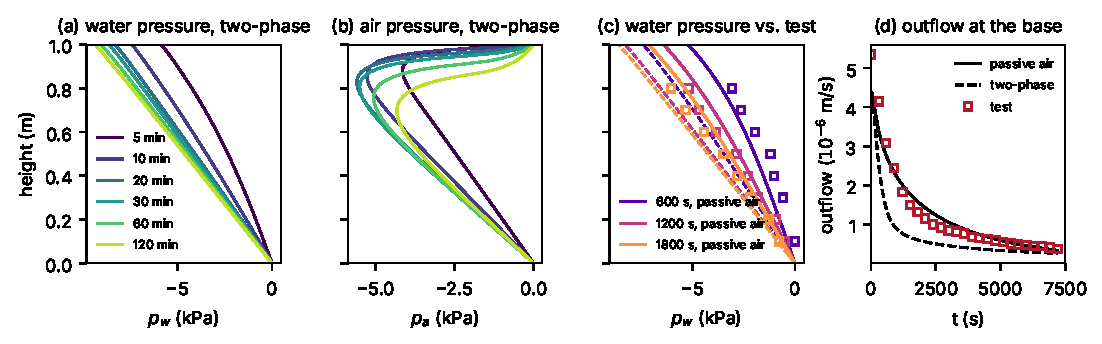
\includegraphics[width=\textwidth]{liakopoulos.pdf}
\caption{Drainage of the Liakopoulos column. (a) Water and (b) air pressure profiles of the two-phase model, with the
solution of \citet{khoei2011} (circles; water pressure at the top and at 0.5~m, minimum air pressure). (c) Water
pressure of the passive-air model (solid) and of the two-phase model (dashed) and the measured values (squares;
\citealp{callari2009}). (d) Outflow at the base and the measured outflow.}\label{fig:liak}
\end{figure}

\begin{table}[htbp]
\centering\small
\caption{Liakopoulos test, two-phase model: NeoPZ and \citet{khoei2011} (values read from their Fig.~1, uncertainty
about 0.15~kPa and 0.03~mm).}\label{tab:liak}
\begin{tabular}{rcccccccc}
\toprule
$t$ & \multicolumn{2}{c}{$p_w$ at the top (kPa)} & \multicolumn{2}{c}{$p_w$ at 0.5 m (kPa)} & \multicolumn{2}{c}{min.\ $p_a$ (kPa)} & \multicolumn{2}{c}{settlement (mm)}\\
(min) & NeoPZ & ref. & NeoPZ & ref. & NeoPZ & ref. & NeoPZ & ref.\\
\midrule
5 & -5.82 & -6.25 & -2.32 & -2.50 & -4.15 & -4.40 & 0.90 & 0.97\\
10 & -7.35 & -7.30 & -3.44 & -3.50 & -5.26 & -5.10 & 1.26 & 1.26\\
20 & -8.22 & -8.00 & -4.03 & -4.00 & -5.57 & -5.30 & 1.45 & 1.40\\
30 & -8.54 & -8.30 & -4.21 & -4.15 & -5.48 & -5.25 & 1.51 & 1.46\\
60 & -8.96 & -8.95 & -4.43 & -4.35 & -5.05 & -5.00 & 1.58 & 1.55\\
120 & -9.29 & -9.25 & -4.60 & -4.55 & -4.33 & -4.30 & 1.62 & 1.60\\
\bottomrule
\end{tabular}

\end{table}

The two-phase solution agrees with that of \citet{khoei2011} (Fig.~\ref{fig:liak}a,b; Table~\ref{tab:liak}): the
water pressure at the top differs by 0.43~kPa (7\%) after 5~min and by less than 0.25~kPa afterwards, the minimum air
pressure, about $-5.5$~kPa near the top where the air enters the drying sand, by less than 0.3~kPa, and the
settlement of the top by less than 0.07~mm. The passive-air solution reproduces the measured outflow and pore
pressures (Fig.~\ref{fig:liak}c,d), as other single-phase solutions do \citep{callari2009}. The two-phase model,
with the usual Brooks--Corey air permeability, drains more slowly than the test; the same happens in the two-phase
solution of \citet{khoei2011}, so this is a feature of the air permeability law and not of the implementation. The test verifies the air phase and the coupling, and shows that, even in drainage, the air resistance
reduces the outflow by a factor of two to three between 10 and 30~min.

\subsection{Reference slope}

The slope of \citet{rahardjo2007} is 10~m high, inclined at $45^\circ$, with 30-m platforms at the crest and at the toe
and the base 20~m below the toe; the initial water table is 5~m below the toe and inclined at $7^\circ$, and the
initial suction is hydrostatic and limited to 75~kPa (Table~\ref{tab:par}, Fig.~\ref{fig:problema}). The standard
mesh has 1684 triangles, with elements of 0.75~m down to 2~m below the surface.

\begin{figure}[htbp]
\centering
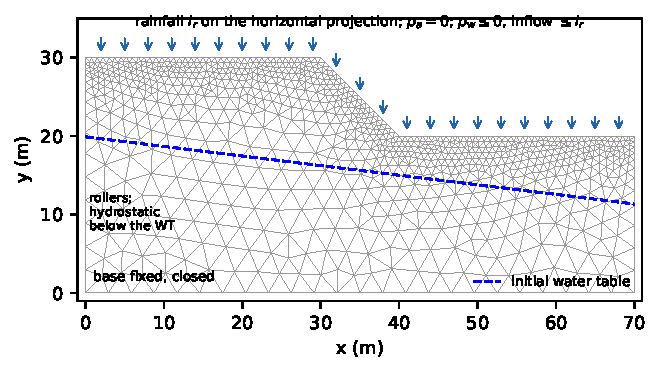
\includegraphics[width=0.9\textwidth]{problema.pdf}
\caption{Reference slope \citep{rahardjo2007}: geometry, standard mesh, initial water table and boundary
conditions.}\label{fig:problema}
\end{figure} The initial FS agrees with that of \citet{rahardjo2007}: 2.119 against 2.11 for the
reference slope and differences of at most 0.05 for heights of 5 to 40~m and water tables 2.5 to 15~m deep; a
simplified Bishop analysis with a search of circular surfaces on the same initial pressures gives 2.092. With model
(iii) the minimum FS under 24-h rainfalls follows the sigmoid fitted by \citet{rahardjo2007} to their results (their
Eq.~6) within 0.01--0.14, the largest differences in the transition between the upper and the lower plateau. The static benchmark of \citet{zhang2014},
which compares six laws for the suction strength, is reproduced within 0--5\%.

\begin{table}[htbp]
\centering\small
\caption{Parameters of the reference slope \citep{rahardjo2007}; $E$, $\nu$, $\psi$ and the air parameters are
assumptions of this study.}\label{tab:par}
\begin{tabular}{p{4.6cm}p{9.6cm}}
\toprule
soils $f_{10}$, $f_{50}$, $f_{100}$ & $a=10$, 50, 100~kPa; $k_s=10^{-4}$, $10^{-5}$, $10^{-6}$~m/s (360, 36 and
3.6~mm/h)\\
retention, $k_{rw}$ & Fredlund--Xing, $n=m=1$, $\theta_s=0.45$; $k_w=k_s S_w^{\,4}$\\
strength & $c'=10$~kPa, $\phi'=26^\circ$, $\chi=1$ ($\phi^b=\phi'$), $\gamma=20$~kN/m$^3$\\
elasticity, dilatancy & $E=20$~MPa, $\nu=0.3$; $\psi=\phi'$ (associated) or $\psi=0$\\
air & Brooks--Corey $\lambda=3$, $k_{ra}^{\min}=10^{-4}$, $\mu_w/\mu_a=55.6$\\
initial state & water table 5~m below the toe, inclined at $7^\circ$; suction $\le75$~kPa\\
rainfall & uniform, 24~h; 48~h simulated\\
\bottomrule
\end{tabular}
\end{table}

%======================================================================
\section{Failure criterion and critical intensity}\label{sec:criterio}
%======================================================================

The slope fails when the FS reaches one. Since the FS of each instant is computed with the pressures of that
instant frozen, a value below one does not describe a physical state: the slope would already have moved and
redistributed the pressures. Below one the FS only measures how far equilibrium has been exceeded. The quantity to
compare is therefore whether, with which rainfall and at which instant, the FS reaches one. We define the critical
intensity $\Ic$ as the smallest intensity of a 24-h rainfall whose minimum FS is $\le1.01$, obtained by linear
interpolation between the computed intensities that bracket it, and the time to failure as the first instant with
FS $\le1.01$ (or $t_f$, if the coupled transient loses equilibrium earlier). The threshold 1.01 accounts for the
resolution of the FS: the bisection tolerance (0.002) and the discretization error, about 0.01 for the standard mesh
(Section~\ref{sec:malha}).

The lower FS plateau of the intense rainfalls, the value that the usual analyses report as the minimum FS, is the FS
of the slope saturated up to its surface with the water flowing through it. A single steady-state calculation with
the surface ponded gives 0.84--0.85 for the three soils, the plateau of model (iii); it is reached after about 7, 24
and 170~h of ponding in the $f_{10}$, $f_{50}$ and $f_{100}$ soils, respectively, and depends on the geometry and on
the orientation of an anisotropic conductivity tensor (0.63--1.05), not on the magnitude of $k_s$. The value 1.45 of
\citet{rahardjo2007} for the $f_{100}$ soil is the FS at the end of 24 h of rainfall, not a plateau. A plateau below
one distinguishes no slopes that have already failed; it only matters when it stays above one, in which case no
rainfall of that duration fails the slope.

%======================================================================
\section{Critical intensity of the reference slope}\label{sec:decomp}
%======================================================================

% Seção 5: intensidade crítica do talude de referência e decomposição do viés (f50, alpha = 45 graus, 24 h)
Figure~\ref{fig:decomp} and Table~\ref{tab:decomp} give the minimum FS under 24-h rainfalls of the $f_{50}$ soil
($k_s=36\mmh$) in the four models, the critical intensities and the times to failure. All the models have a critical
intensity: from $\Ic$ on, the FS reaches one during the rainfall and does not rise again while it rains
(Fig.~\ref{fig:fstempo}). In this sense the limiting intensity of \citet{rahardjo2007} exists in every model. What
changes is its value. The usual model (iii) gives $\Ic=48\mmh$ ($1.3k_s$); the complete model (i) gives 31~mm/h
($0.9k_s$) with an associated flow rule and 26~mm/h ($0.7k_s$) without dilatancy. The hypotheses of the usual chain
overestimate by 54 to 86\% the rainfall that brings the slope to failure; against the sigmoid published by
\citet{rahardjo2007}, which reaches one at about 40~mm/h, by 28 to 54\%. They also delay the failure: with 54~mm/h
the FS of model (iii) reaches one after 22~h, against 18~h in model (i) with $\psi=\phi'$ and the loss of equilibrium
after 12.5~h with $\psi=0$; with 90~mm/h, after 20, 18 and 12~h.

\begin{figure}[htbp]
\centering
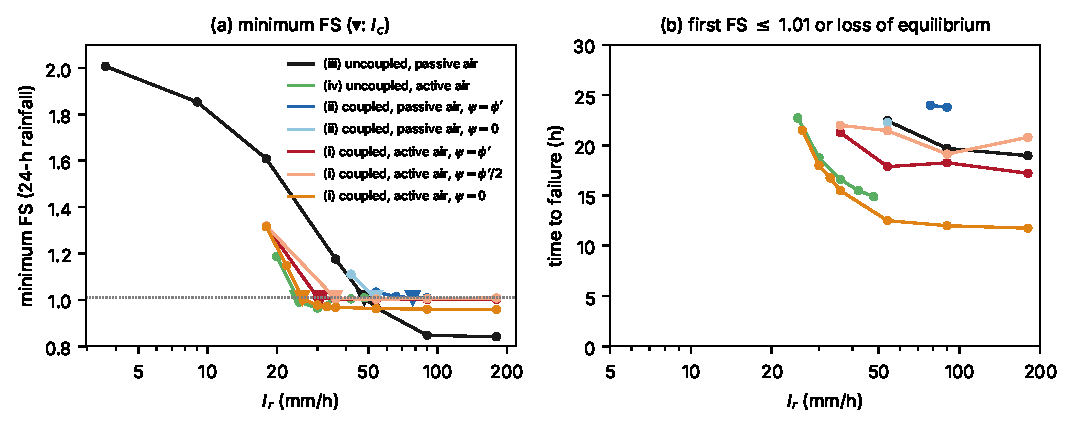
\includegraphics[width=\textwidth]{decomposicao.pdf}
\caption{Soil $f_{50}$, $\alpha=45^\circ$, 24-h rainfalls. (a) Minimum FS against the rainfall intensity in the
four models ($\blacktriangledown$: critical intensity, FS $=1.01$). (b) Time to failure: first instant with FS
$\le1.01$, or loss of equilibrium of the coupled transient with $\psi=0$.}\label{fig:decomp}
\end{figure}

\begin{table}[htbp]
\centering\footnotesize\setlength{\tabcolsep}{4pt}
\caption{Critical intensity ($k_s=36\mmh$) and time to failure of the reference slope. Bracket: computed intensities
on each side of $\Ic$ (FS $\le1.01$); the column FS $\le1.02$ gives $\Ic$ with that threshold. Time to failure: first
instant with FS $\le1.01$; --: no failure; blank: not computed. $^\dagger$Loss of equilibrium of the coupled
transient.}\label{tab:decomp}
\begin{tabular}{lcccccccc}
\toprule
model & $I_c$ & bracket & $I_c/k_s$ & $I_c$ & \multicolumn{4}{c}{time to failure (h) for $I_r$ (mm/h) $=$}\\
 & (mm/h) & (mm/h) & & FS $\le1.02$ & 36 & 48 & 54 & 90\\
\midrule
(iii) uncoupled, passive air & 48 & 48--54 & 1.33 & 47 & -- & -- & 22.4 & 19.7\\
(iv) uncoupled, active air & 25 & 20--25 & 0.69 & 25 & 16.6 & 14.9 &  & \\
(ii) coupled, passive, $\psi=\phi'$ & 78 & 66--78 & 2.16 & 62 &  &  & -- & \\
(ii) coupled, passive, $\psi=0$ & 53 & 42--54 & 1.49 & 52 &  &  & 22.2$^\dagger$ & \\
(i) coupled, active, $\psi=\phi'$ & 31 & 30--36 & 0.86 & 30 & 21.3 &  & 17.9 & 18.3\\
(i) coupled, active, $\psi=\phi'/2$ & 36 & 18--36 & 0.99 & 35 & 22.0 &  & 21.5 & 19.1\\
(i) coupled, active, $\psi=0$ & 26 & 22--26 & 0.72 & 26 & 15.5$^\dagger$ &  & 12.5$^\dagger$ & 12.0$^\dagger$\\
\bottomrule
\end{tabular}

\end{table}

The four models separate the two hypotheses (Table~\ref{tab:decomp}).
\begin{itemize}
\item \emph{The air lowers the critical intensity by about half}: on a rigid skeleton from 48 to 25~mm/h (passive and
active air, models iii and iv); in the coupled models from 53 to 26~mm/h without dilatancy and from 78 to 31~mm/h
with $\psi=\phi'$ (from 62 to 30~mm/h with the threshold 1.02).
\item \emph{The coupling raises it}: by 4--10\% without dilatancy (from 25 to 26~mm/h with active air, from 48 to
53~mm/h with passive air) and by 24--63\% with associated dilatancy (to 31 and 78~mm/h). The deformation of the
skeleton during the wetting, elastic swelling as the effective stress decreases and plastic dilation in the shear
zone, opens pore space and lowers the pore pressures.
\end{itemize}
The two simplifications of the usual model thus have opposite effects: neglecting the deformation is conservative,
neglecting the air is not, and the air dominates. A two-phase flow analysis on a rigid skeleton, model (iv), recovers
the bias: its critical intensity, 25~mm/h, is 4\% below that of the complete model without dilatancy and 20\% below
that with associated dilatancy, and its time to failure with 36~mm/h, 16.6~h, lies between those of the complete model
with $\psi=0$ (15.5~h) and with $\psi=\phi'$ (21.3~h).

The coupled models with an associated flow rule approach one from above (1.000--1.014 for $I_r\ge\Ic$), so their
critical intensity depends on the threshold. With FS $\le1.02$ instead of 1.01 the critical intensities change by
less than 1~mm/h, except that of model (ii) with $\psi=\phi'$, whose minimum FS is 1.033, 1.014 and 1.010 with 54, 66
and 78~mm/h: $\Ic=62$ instead of 78~mm/h. In this model the slope sits in limit equilibrium over a wide range of
intensities, with plastic deformation but without loss of equilibrium.


%======================================================================
\section{Trapped air}\label{sec:ar}
%======================================================================

% Seção 6: ar aprisionado (f100, alpha = 63,4 graus; confinamento, k_ra,min, malha)
\citet[pp.~1539, 1541]{rahardjo2007} conclude that slopes with $k_s\le10^{-6}$~m/s, ``even when the rainfall intensity
is extremely high'', do not fail under rainfalls of up to 24~h, because the rain does not raise the water table and
most of it runs off. We examine the $f_{100}$ soil ($k_s=3.6\mmh$) on the steepest slope of their study,
$\alpha=63.4^\circ$, whose initial FS is 1.775 in our analysis (Fig.~\ref{fig:ar}); their Fig.~9c gives about 1.69
for the initial FS and about 1.12 and 1.05 for the minimum FS with 9 and 80~mm/h (read from the figure). With the
usual model (iii) the minimum FS under 24-h rainfalls is 1.383, 1.163, 1.097 and 1.093 for $I_r=9$, 18, 36 and
80~mm/h: the slope does not fail, as \citet{rahardjo2007} conclude. With model (ii) the minimum FS is 0.015--0.041
higher. With active air (model i) it is 1.166, 1.028, 1.015 and 1.013: from 36~mm/h on, the minimum FS is within 0.02
of one at the end of the rainfall, i.e.\ the slope fails with $\delta=0.02$ ($I_{c,0.02}=29$~mm/h) but not with
$\delta=0.01$. With elements of 0.35~m near the surface the minimum FS with 36~mm/h is 1.009 (Section~\ref{sec:malha}).

\begin{figure}[htbp]
\centering
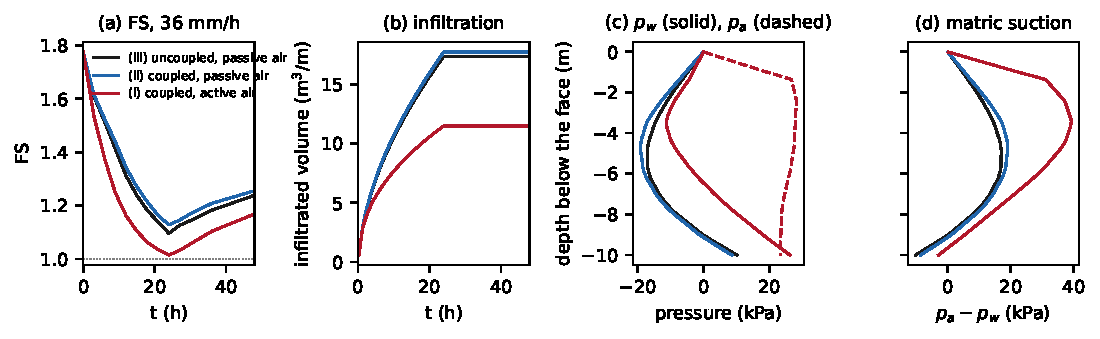
\includegraphics[width=\textwidth]{ar_aprisionado.pdf}
\caption{Soil $f_{100}$, $\alpha=63.4^\circ$, $I_r=36\mmh$ during 24~h, in models (i)--(iii). (a) FS; (b) infiltrated
volume; (c) water (solid) and air (dashed, model i) pressures and (d) matric suction along a vertical below the
middle of the face at $t=24$~h.}\label{fig:ar}
\end{figure}

The lower FS of model (i) is not associated with more water. With active air 10.4--11.6~m$^3$/m infiltrate in 24~h,
against 13.5--18.0~m$^3$/m with passive air (Fig.~\ref{fig:ar}b). The surface ponds earlier with active air: with
9~mm/h the first vertex ponds after 6~h with active air and after 11.75~h with passive air, and at the end of the
rainfall 83 and 41 of the 96 surface vertices are ponded; with 36~mm/h the whole surface ponds within 4.5~h with
active air and 6.5~h with passive air. With 36~mm/h the maximum air pressure is 19.5~kPa after 1~h, 30~kPa after 3~h
and 38~kPa after 24~h. At the end of the rainfall, along a vertical below the middle of the face
(Fig.~\ref{fig:ar}c,d), the air pressure averages 32~kPa between 0.5 and 5~m of depth; between 2 and 5~m the matric
suction is 38~kPa with active air and 24~kPa with passive air, and the water pressure is $-6\kpa$ with active air
and $-24\kpa$ with passive air. The matric suction is therefore higher with active air, while the water pressure,
which with $\chi=1$ is the only pressure in the effective stress (Eq.~\ref{eq:bishop}), is also higher. Across the
models, a smaller infiltrated volume comes with a smaller FS. \citet[p.~1539]{rahardjo2007} relate the decrease of
the minimum FS to the rainfall volume needed to initiate and to complete it; within each of our models the minimum FS
also decreases with the intensity, but between models with and without active air the ordering of volume and FS is
reversed.

The air pressure depends on how easily the air leaves through the ponded surface. With the minimum relative
permeability of the air $k_{ra}^{\min}$ between $10^{-6}$ and $10^{-3}$ the minimum FS is 1.013--1.015 and the maximum
air pressure 37--38~kPa; with $10^{-2}$ the air pressure falls to 28~kPa and the minimum FS rises to 1.046.

\subsection{Confinement of the air}\label{sec:confinamento}

The base and the lateral boundaries are closed to the air in the reference model. Opening them (atmospheric air
pressure on the base and on the lateral boundaries) changes the minimum FS by less than 0.002: 1.017 against 1.015 for
the $f_{100}$ slope with 36~mm/h, and 1.011 against 1.011 for the $f_{50}$ slope with 30~mm/h. The lateral boundaries
are 30~m away from the slope and the base is below the water table.

\subsection{Mesh}\label{sec:malha}

The minimum FS of the $f_{100}$ slope with 36~mm/h decreases with the mesh: 1.0154, 1.0122 and 1.0090 with elements
of 0.75, 0.5 and 0.35~m near the surface (1620, 3597 and 7314 triangles), by about 0.003 per refinement, while the
initial FS changes less at each refinement (1.775, 1.761 and 1.752; Fig.~\ref{fig:malha}). Whether the converged
minimum FS falls below one cannot be decided with these meshes.

\begin{figure}[htbp]
\centering
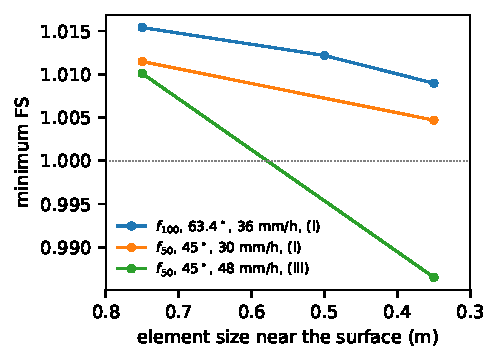
\includegraphics[width=0.5\textwidth]{malha.pdf}
\caption{Minimum FS against the element size near the surface: $f_{100}$ slope at $63.4^\circ$ with 36~mm/h in model
(i), and the $f_{50}$ reference slope near its critical intensities in models (i) and (iii).}\label{fig:malha}
\end{figure}


%======================================================================
\section{Dilatancy and the response after failure}\label{sec:dilat}
%======================================================================

% Seção 7: dilatância e resposta depois da ruptura
The dilatancy changes the critical intensity and, above all, what the coupled transient does after it
(Figs.~\ref{fig:fstempo} and \ref{fig:decomp}). Without dilatancy ($\psi=0$) the coupled transient of model (i) loses
equilibrium for $I_r\ge26\mmh$, between 21.5~h (26~mm/h) and 11.75~h (180~mm/h); with 22~mm/h it does not. With
$\psi=\phi'/2$ or $\psi=\phi'$ the minimum FS stays between 1.000 and 1.008 from 36 to 180~mm/h and the transient never
loses equilibrium: the slope is at limit equilibrium, within the resolution of the FS, without collapse of the
transient. Below the critical intensity the flow rule hardly matters: with 18~mm/h the minimum FS is 1.316 with
$\psi=0$ and 1.319 with $\psi=\phi'/2$ and $\phi'$. With $\delta=0.01$ the critical intensity is 26~mm/h with $\psi=0$
and 31~mm/h with $\psi=\phi'$ (20\% higher); with $\psi=0$ the failure occurs 5.4--6.3~h earlier in the rainfalls of 54
and 90~mm/h (Table~\ref{tab:decomp}). With $\psi=\phi'/2$ only 18 and 36~mm/h were computed below 54~mm/h, so its
critical intensity is only known to lie between 18 and 36~mm/h.

\begin{figure}[htbp]
\centering
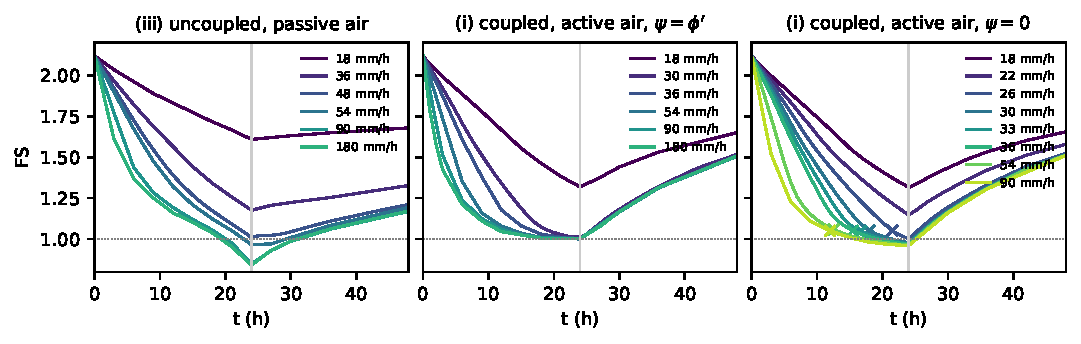
\includegraphics[width=\textwidth]{fs_tempo.pdf}
\caption{FS during and after 24-h rainfalls of several intensities, soil $f_{50}$, $\alpha=45^\circ$: model (iii)
and model (i) with $\psi=\phi'$ and $\psi=0$ ($\times$: loss of equilibrium of the coupled transient; afterwards the
transient continues with the strength increased, only to follow the pressures).}\label{fig:fstempo}
\end{figure}

With $\psi=0$ the loss of equilibrium occurs when the FS of the strength reduction, computed with $\psi=\phi'$, is
still 1.047--1.059. Either the associated strength reduction overestimates by about 5\% the FS of a soil without
dilatancy, or part of the loss of equilibrium is numerical; the time step does not explain it: with a time step of
0.125~h instead of 0.25~h during the rainfall, the transient with 36~mm/h loses equilibrium after 15.6~h instead of
15.5~h. For $\psi=0$ the time of failure is therefore $t_f$, and $22<\Ic\le26\mmh$ by the loss of equilibrium. The
FS values below one after $t_f$ use the pressures of a transient continued with the strength increased and only show
that the equilibrium was exceeded.

The flow rule matters as much with passive air. In model (ii) the transient without dilatancy loses equilibrium
after 22.3~h with 54~mm/h, and its critical intensity is 53~mm/h; with $\psi=\phi'$ the minimum FS is 1.033, 1.014,
1.010 and 1.009 with 54, 66, 78 and 90~mm/h, and the transient never loses equilibrium. In both coupled models,
the transients with an associated flow rule do not collapse in the range computed, and those without dilatancy do. The
mechanism (for instance the suction generated by the plastic dilation of the shear zone) was not isolated here.


%======================================================================
\section{Generalization}\label{sec:gen}
%======================================================================

% Seção 8: generalização (solo, lei de chi, geometria, confinamento, malha)
Table~\ref{tab:gen} extends the comparison of models (i) and (iii) to the permeable $f_{10}$ soil, to the Bishop
parameter $\chi=S_e$ and to the low-permeability $f_{100}$ soil on two slopes.

\begin{table}[htbp]
\centering\small
\caption{Critical intensity (mm/h) of 24-h rainfalls in the usual model (iii) and in the complete model (i,
$\psi=\phi'$). $>$: no failure up to the most intense rainfall computed, whose minimum FS is given in
parentheses; $^\ast$limit equilibrium (minimum FS $\le1.02$).}\label{tab:gen}
\begin{tabular}{lc ccccc ccccc}
\toprule
 & & \multicolumn{5}{c}{model (iii)} & \multicolumn{5}{c}{model (i), $\psi=\phi'$}\\
\cmidrule(lr){3-7}\cmidrule(lr){8-12}
slope and soil & $k_s$ & 0.02 & 0.01 & 0.005 & 0 & min.\ FS & 0.02 & 0.01 & 0.005 & 0 & min.\ FS\\
\midrule
$f_{50}$, $45^\circ$, $\chi=1$ (reference) & 36 & 47 & 48 & 49 & 49 & 0.841 & 30 & 31 & 35 & $>180$ & 1.000\\
$f_{10}$, $45^\circ$, $\chi=1$ & 360 & $\le$129 & $\le$135 & $\le$138 & n.c. & 0.841 & $\le$129 & $\le$139 & n.c. & n.c. & 1.029\\
$f_{50}$, $45^\circ$, $\chi=S_e$ & 36 & 47 & $\le$48 & $\le$51 & $\le$53 & 1.010 & $\le$27 & $\le$30 & n.c. & n.c. & 1.034\\
$f_{100}$, $63.4^\circ$, $\chi=1$ & 3.6 & $>80$ & $>80$ & $>80$ & $>80$ & 1.093 & 29 & $>80$ & $>80$ & $>80$ & 1.013\\
$f_{100}$, $45^\circ$, $H_s=20$~m, $\chi=1$ & 3.6 & $>80$ & $>80$ & $>80$ & $>80$ & 1.252 & $>80$ & $>80$ & $>80$ & $>80$ & 1.172\\
\bottomrule
\end{tabular}

\end{table}

\emph{Permeable soil.} In the $f_{10}$ soil ($k_s=360\mmh$) the critical intensity is 135~mm/h in model (iii) and
139~mm/h in model (i): the bias of the usual model disappears. The critical intensities are well below $k_s$
($0.4k_s$), the surface does not pond before the slope fails and the air escapes through it. The bias is a feature
of the regime $\Ic\gtrsim k_s$, in which the surface seals the air: in the $f_{50}$ soil $\Ic$ of model (iii) is
$1.3k_s$.

\emph{Low-permeability soil.} In the $f_{100}$ soil ($k_s=3.6\mmh$) no 24-h rainfall of up to 80~mm/h brings a
20-m, $45^\circ$ slope to failure in either model; the complete model gives a minimum FS 0.08--0.11 lower (1.17
against 1.25 with 80~mm/h), and its minimum occurs after the rainfall, 30--36~h after its start. On the $63.4^\circ$ slope the usual model stays
9--10\% above failure at any intensity, whereas the complete model reaches limit equilibrium (Section~\ref{sec:ar}).
For this soil the comparison is not a shift of $\Ic$ but the difference between a safe slope and one at the limit.

\emph{Bishop parameter.} With $\chi=S_e$ (for the Fredlund--Xing curve with $C(\psi)=1$, $S_e=S_w$) the suction
contributes less to the initial strength (initial FS 1.895 instead of 2.119) and the air pressure also enters the
effective stress, through $(1-\chi)p_a$. The critical intensity of model (iii) is unchanged, 48~mm/h (minimum FS
1.010 and 0.998 with 48 and 54~mm/h), and that of model (i) falls from 31 to 30~mm/h: the bias persists (+62\%). Near
failure the controlling zone is nearly saturated and $\chi\to1$ in both laws, so the law of $\chi$ changes the
initial FS much more than the critical intensity.

\emph{Confinement of the air.} Opening the base and the lateral boundaries to the air changes the minimum FS by less
than 0.002 (Section~\ref{sec:confinamento}): the air is sealed by the ponded surface, not by the boundaries of the
domain.

\emph{Mesh.} With elements of 0.35~m instead of 0.75~m near the surface (8052 elements instead of 1834; initial FS
2.106 instead of 2.119), the minimum FS of model (i) with 30~mm/h falls from 1.011 to 1.005 and that of model (iii)
with 48~mm/h from 1.010 to 0.987 (Fig.~\ref{fig:malha}). With the local slope of the minimum FS with the intensity
these differences shift the critical intensities to about 30 and 46~mm/h; the ratio between them, 1.5, does not
change.


%======================================================================
\section{Implications for rainfall thresholds}\label{sec:impl}
%======================================================================

% Seção 9: consequências para limiares de chuva
Physically based rainfall thresholds are the critical intensities of the analyses, for a set of durations. For the
reference slope, the usual model places the 24-h threshold at $1.3k_s$; the complete model at $0.9k_s$ with an
associated flow rule and $0.7k_s$ without dilatancy. A threshold derived from the usual chain is thus not
conservative: rainfalls between the two thresholds, which the usual analysis classifies as safe, bring the slope to
failure. In a probabilistic setting, where the annual failure probability integrates the conditional probability of
failure over the intensity--frequency distribution of the rainfall \citep[e.g.][]{tang2018}, the shift of the
threshold changes the exceedance probability of the failure-triggering rainfall by a factor that depends on the
local intensity--duration--frequency curve; for a 24-h rainfall, a threshold 35--46\% lower corresponds to a much
more frequent event.

Two of the conclusions of \citet{rahardjo2007} change with the failure criterion and the complete model. (1) Low
permeability does not guarantee safety under short rainfalls: the trapped air brings the $f_{100}$ slope at
$63.4^\circ$ to limit equilibrium in 24~h, a slope that the usual analysis places 9--10\% above failure. (2) The
limiting intensity and the lower plateau are not properties of the soil: the plateau is the FS of the slope saturated
to its surface and can be computed directly, with a single steady-state calculation with the surface ponded, without
simulating the rainfall; whether the slope fails depends on whether that value is below one.

When is the usual model enough? The bias comes from the air sealed below a ponded surface. For rainfall intensities
well below $k_s$ the surface does not pond before the slope fails, the air escapes and the usual model gives the
critical intensity of the complete one (135 and 139~mm/h for the $f_{10}$ soil). The bias concentrates in the regime
$\Ic\gtrsim k_s$, in which the surface ponds early, which is the regime of the critical intensities of the $f_{50}$
and $f_{100}$ soils. In that regime a two-phase flow analysis on a rigid skeleton
recovers the bias and errs on the safe side by 4--20\% (model iv); the usual single-phase seepage analysis does not.


%======================================================================
\section{Limitations}\label{sec:lim}
%======================================================================

\begin{itemize}
\item Two-dimensional, homogeneous slope with a single geometry for the decomposition; the critical intensity of
other slopes was examined only for two soils, two Bishop laws and one steeper slope.
\item The air leaves only through the ground surface, and once it ponds only through the minimum relative
permeability $k_{ra}^{\min}$. Opening the base and the lateral boundaries does not change the results
(Section~\ref{sec:confinamento}), but real slopes have macropores, cracks, vegetation and heterogeneities that let
the air out through a ponded surface; their effect is represented here only by $k_{ra}^{\min}$, and with
$k_{ra}^{\min}=10^{-2}$ the FS rises by 0.035.
\item The strength reduction is associated even when the transient uses $\psi=0$; the loss of equilibrium of the
transient is then the failure indicator, and part of it may be numerical.
\item No hysteresis of the retention curve, constant porosity in the hydraulic coefficients, no dissolved air, no
vapour and an isothermal ideal gas.
\item The mesh error of the FS was assessed in three cases (Fig.~\ref{fig:malha}): with 0.35-m elements the minimum
FS falls by 0.007--0.024 and, in the $f_{100}$ case, by about 0.003 per refinement without clear convergence; the
critical intensities shift by 1--2~mm/h.
\item The air phase was validated in drainage (Liakopoulos), not in infiltration with air entrapment; a validation
against a column with measured air pressure under infiltration \citep{toumavauclin1986} is still needed.
\end{itemize}

%======================================================================
\section{Conclusions}\label{sec:concl}
%======================================================================

% Seção 11: conclusões
A coupled formulation with displacement, pore-water and pore-air pressures was implemented in NeoPZ, validated against
the Liakopoulos drainage test and used to quantify how the hypotheses of the usual chain of analysis, uncoupled
seepage with atmospheric pore air followed by a stability analysis with the frozen pressures, bias the rainfall that
brings an unsaturated slope to failure. The main conclusions are the following.
\begin{enumerate}
\item With the failure criterion FS $\le1$, models must be compared by the critical intensity and the time to
failure, not by the minimum FS. A minimum FS below one is the FS of the slope saturated to its surface, a property
of the boundary-value problem that can be computed directly with the surface ponded.
\item For the homogeneous slope of \citet{rahardjo2007} with $k_s=36\mmh$ the usual model gives a critical intensity
of 48~mm/h ($1.3k_s$) for 24-h rainfalls, and the complete model 31~mm/h ($0.9k_s$) with an associated flow rule and
26~mm/h ($0.7k_s$) without dilatancy. The usual hypotheses overestimate the failure-triggering rainfall by 54--86\%
and delay the predicted failure by up to 10~h in intense rainfalls. The bias persists with $\chi=S_e$ (48 against
30~mm/h) and with a finer mesh (about 46 against 30~mm/h).
\item The two simplifications act in opposite directions. The trapped air halves the critical intensity; the coupling
raises it, by 4--10\% through the elastic swelling of the skeleton and by up to 63\% when the plastic dilation of an
associated flow rule is added. The air dominates, and a two-phase flow analysis on a rigid skeleton recovers the bias
with a critical intensity 4--20\% below that of the complete model.
\item The trapped air lowers the FS with less water. Once the surface ponds, the air between the wetting front and
the water table is compressed to 36--38~kPa; less water infiltrates and the matric suction increases, but the
pore-water pressure rises with the air pressure and the effective stress falls. A low-permeability slope
($k_s=3.6\mmh$, $63.4^\circ$) that the usual model places 9--10\% above failure reaches limit equilibrium; the effect
does not depend on whether the base and lateral boundaries are open to the air.
\item Dilatancy does not decide whether a critical intensity exists but shifts it by about 20\% and decides the
response after it is exceeded: without dilatancy the coupled transient loses equilibrium, independently of the time
step; with $\psi\ge\phi'/2$ the slope stays at limit equilibrium.
\item The bias concentrates in the regime $\Ic\gtrsim k_s$, in which the surface ponds and seals the air. For a
permeable soil whose critical intensity is well below $k_s$ the usual model is adequate (135 against 139~mm/h).
\end{enumerate}
Rainfall thresholds derived from uncoupled, passive-air analyses are therefore unconservative for slopes whose
critical rainfall exceeds the saturated conductivity of the surface soil. The validation of the air phase in
infiltration with measured air pressures, natural (open, heterogeneous) slopes and three-dimensional effects are the
next steps.


\section*{Code and data availability}
The material \texttt{TPZMatUnsaturatedUPwPa}, the program \texttt{SlopeRainfall} and the scripts that run all the
cases and draw the figures are part of the NeoPZ library (\url{https://github.com/labmec/neopz}); the results are in
\texttt{Projects/SlopeRainfall/resultados}.

\bibliographystyle{elsarticle-harv}
\begin{thebibliography}{99}
% Lista de referências (entradas marcadas com %VERIFICAR: conferir volume e páginas antes da submissão)
\bibitem[Bishop(1959)]{bishop1959}
Bishop, A.W., 1959. The principle of effective stress. Teknisk Ukeblad 106(39), 859--863.

\bibitem[Caine(1980)]{caine1980}
Caine, N., 1980. The rainfall intensity--duration control of shallow landslides and debris flows. Geografiska
Annaler A 62, 23--27.

\bibitem[Callari and Abati(2009)]{callari2009}
Callari, C., Abati, A., 2009. Finite element methods for unsaturated porous solids and their application to dam
engineering problems. Computers \& Structures 87, 485--501.

\bibitem[Celia et~al.(1990)]{celia1990}
Celia, M.A., Bouloutas, E.T., Zarba, R.L., 1990. A general mass-conservative numerical solution for the unsaturated
flow equation. Water Resources Research 26(7), 1483--1496.

\bibitem[Cho(2016)]{cho2016}
Cho, S.E., 2016. Stability analysis of unsaturated soil slopes considering water-air flow caused by rainfall
infiltration. Engineering Geology 211, 184--197. %VERIFICAR

\bibitem[Devloo(1997)]{devloo1997}
Devloo, P.R.B., 1997. PZ: an object oriented environment for scientific programming. Computer Methods in Applied
Mechanics and Engineering 150, 133--153.

\bibitem[Fredlund et~al.(1978)]{fredlund1978}
Fredlund, D.G., Morgenstern, N.R., Widger, R.A., 1978. The shear strength of unsaturated soils. Canadian
Geotechnical Journal 15, 313--321.

\bibitem[Fredlund and Xing(1994)]{fredlund1994}
Fredlund, D.G., Xing, A., 1994. Equations for the soil-water characteristic curve. Canadian Geotechnical Journal
31, 521--532.

\bibitem[Griffiths and Lane(1999)]{griffiths1999}
Griffiths, D.V., Lane, P.A., 1999. Slope stability analysis by finite elements. G\'eotechnique 49(3), 387--403.

\bibitem[Guzzetti et~al.(2008)]{guzzetti2008}
Guzzetti, F., Peruccacci, S., Rossi, M., Stark, C.P., 2008. The rainfall intensity--duration control of shallow
landslides and debris flows: an update. Landslides 5, 3--17.

\bibitem[Khoei and Mohammadnejad(2011)]{khoei2011}
Khoei, A.R., Mohammadnejad, T., 2011. Numerical modeling of multiphase fluid flow in deforming porous media: a
comparison between two- and three-phase models for seismic analysis of earth and rockfill dams. Computers and
Geotechnics 38, 142--166.

\bibitem[Leong and Rahardjo(1997)]{leong1997}
Leong, E.C., Rahardjo, H., 1997. Permeability functions for unsaturated soils. Journal of Geotechnical and
Geoenvironmental Engineering 123(12), 1118--1126.

\bibitem[Lewis and Schrefler(1998)]{lewis1998}
Lewis, R.W., Schrefler, B.A., 1998. The Finite Element Method in the Static and Dynamic Deformation and
Consolidation of Porous Media, 2nd ed. Wiley, Chichester.

\bibitem[Liakopoulos(1965)]{liakopoulos1965}
Liakopoulos, A.C., 1965. Transient flow through unsaturated porous media. PhD thesis, University of California,
Berkeley.

\bibitem[Liu and Wang(2021)]{liu2021}
Liu, X., Wang, Y., 2021. Probabilistic simulation of entire process of rainfall-induced landslides using random
finite element and material point methods with hydro-mechanical coupling. Computers and Geotechnics 132, 103989.

\bibitem[Ng and Shi(1998)]{ng1998}
Ng, C.W.W., Shi, Q., 1998. A numerical investigation of the stability of unsaturated soil slopes subjected to
transient seepage. Computers and Geotechnics 22(1), 1--28.

\bibitem[Pradhan et~al.(2022)]{pradhan2022}
Pradhan, S., Toll, D.G., Rosser, N.J., Brain, M.J., 2022. An investigation of the combined effect of rainfall and
road cut on landsliding. Engineering Geology 307, 106787.

\bibitem[Qi and Vanapalli(2015)]{qi2015}
Qi, S., Vanapalli, S.K., 2015. Hydro-mechanical coupling effect on surficial layer stability of unsaturated
expansive soil slopes. Computers and Geotechnics 70, 68--82. %VERIFICAR

\bibitem[Rahardjo et~al.(2007)]{rahardjo2007}
Rahardjo, H., Ong, T.H., Rezaur, R.B., Leong, E.C., 2007. Factors controlling instability of homogeneous soil slopes
under rainfall. Journal of Geotechnical and Geoenvironmental Engineering 133(12), 1532--1543.

\bibitem[Schrefler and Scotta(2001)]{schrefler2001}
Schrefler, B.A., Scotta, R., 2001. A fully coupled dynamic model for two-phase fluid flow in deformable porous media.
Computer Methods in Applied Mechanics and Engineering 190, 3223--3246.

\bibitem[Tang et~al.(2018)]{tang2018}
Tang, G., Huang, J., Sheng, D., Sloan, S.W., 2018. Stability analysis of unsaturated soil slopes under random
rainfall patterns. Engineering Geology 245, 322--332.

\bibitem[Touma and Vauclin(1986)]{toumavauclin1986}
Touma, J., Vauclin, M., 1986. Experimental and numerical analysis of two-phase infiltration in a partially saturated
soil. Transport in Porous Media 1, 27--55.

\bibitem[Tschuchnigg et~al.(2015)]{tschuchnigg2015}
Tschuchnigg, F., Schweiger, H.F., Sloan, S.W., 2015. Slope stability analysis by means of finite element limit
analysis and finite element strength reduction techniques. Part I: Numerical studies considering non-associated
plasticity. Computers and Geotechnics 70, 169--177. %VERIFICAR

\bibitem[Wang et~al.(2018)]{wang2018mpm}
Wang, B., Vardon, P.J., Hicks, M.A., 2018. Rainfall-induced slope collapse with coupled material point method.
Engineering Geology 239, 1--12.

\bibitem[Yang et~al.(2017)]{yang2017}
Yang, K.H., Uzuoka, R., Thuo, J.N., Lin, G.L., Nakai, Y., 2017. Coupled hydro-mechanical analysis of two unstable
unsaturated slopes subject to rainfall infiltration. Engineering Geology 216, 13--30. %VERIFICAR

\bibitem[Zhang et~al.(2014)]{zhang2014}
Zhang, L.L., Fredlund, D.G., Fredlund, M.D., Wilson, G.W., 2014. Modeling the unsaturated soil zone in slope
stability analysis. Canadian Geotechnical Journal 51, 1384--1398.

\bibitem[Zienkiewicz et~al.(1975)]{zienkiewicz1975}
Zienkiewicz, O.C., Humpheson, C., Lewis, R.W., 1975. Associated and non-associated visco-plasticity and plasticity in
soil mechanics. G\'eotechnique 25(4), 671--689.

\end{thebibliography}

\end{document}
